\documentclass[9pt, serif]{beamer}

% This file is a solution template for:

% - Talk at a conference/colloquium.
% - Talk length is about 20min.
% - Style is ornate.

\usepackage{psfrag}
\usepackage{graphics}
\usepackage{latexsym}
\usepackage{amsfonts}
\usepackage{amsmath}  
\usepackage{bm}
\usepackage{epstopdf}
\usepackage[noend]{algpseudocode}

\newcommand{\Real}{\mathbb R}
\newcommand{\Nat}{\mathbb N}

\newcommand{\la}{\langle}
\newcommand{\ra}{\rangle}
\newcommand{\lp}{\left(}
\newcommand{\rp}{\right)}

\newcommand{\sh}{\Delta}
\newcommand{\kmn}{\frac{(2m+1)!(2n-m)!}{(2n+m+1)!}}

\newcommand{\newpar}{\vspace{.1in}\noindent}

\newcommand{\ds}{\displaystyle}

\newcommand{\bi}{\begin{itemize}}
\newcommand{\be}{\begin{enumerate}}
\newcommand{\ei}{\end{itemize}}
\newcommand{\ee}{\end{enumerate}}

\newcommand{\bfr}[1]{\begin{frame}{\hspace{50mm}#1}}
\newcommand{\efr}{\end{frame}}

\newcommand*\Let[2]{\State #1 $\gets$ #2}

\newcommand{\abs}[1]{\left|#1\right|}

\definecolor{royalblue}{rgb}{.2,.6,1}%
\definecolor{mygrey}{rgb}{.64,.64,.64}%
\definecolor{mywhite}{rgb}{1,1,1}%
\definecolor{mypurple}{rgb}{.8,.6,1}%

\definecolor{red}{rgb}{1,0,0}
\definecolor{skyblue}{rgb}{0.1960, 0.6000, 0.8000}


\mode<presentation>
{
% THEME CHOICES
%\usetheme{CambridgeUS}
\usetheme{Warsaw}
%\usetheme{Rochester}
%\usetheme{Bergen}
%\usetheme{Berlin}
%\usetheme{Copenhagen}
%\usetheme{Boadilla}
%\usetheme{PaloAlto}

% SET BACKGROUND COLORS

\setbeamercolor{background canvas}{bg=white}
\setbeamerfont{frametitle}{size=\large}
}

\setbeamercolor{frame}{bg=mygold}

\usepackage[english]{babel}

\usepackage[latin1]{inputenc}

\usepackage{helvet}
\usepackage[T1]{fontenc}
\title[Secant method]
{More Fun with Roots: the Secant Method}



\author[]
{Nate DeMaagd, Kurt O'Hearn}


\institute[Grand Valley State University]
{MTH 499-02}
  
  \date{February 4, 2013}


% If you have a file called "university-logo-filename.xxx", where xxx
% is a graphic format that can be processed by latex or pdflatex,
% resp., then you can add a logo as follows:

\pgfdeclareimage[height=1cm, width=1cm]{GVlogo}{GVSULOGOBLACK}
 \logo{\pgfuseimage{GVlogo}}

% to mask background in logo image
% \pgfdeclaremask{logobacking}{image name }
%


% Delete this, if you do not want the table of contents to pop up at
% the beginning of each subsection:
%\AtBeginSubsection[]
%{
 % \begin{frame}<beamer>{Outline}
 %   \tableofcontents[currentsection,currentsubsection]
 % \end{frame}
%}


% If you wish to uncover everything in a step-wise fashion, uncomment
% the following command:

%\beamerdefaultoverlayspecification{<+->}

\begin{document}

\begin{frame}
  \titlepage
\end{frame}

%\begin{frame}{Outline}
 % \tableofcontents
  % You might wish to add the option [pausesections]
%\end{frame}


%SLIDE 1
\begin{frame}{\hspace{50mm}Introduction}
    \LARGE{Our outline for today is\ldots }
    \pause
    \bi
        \item Definition and graphical interpretation of the secant method
        \pause
        \item Pseudocode
        \pause
        \item Error analysis and convergence rate
        \pause
        \item Implementation and examples
    \ei
\end{frame}

%SLIDE 2
\begin{frame}{\hspace{50mm}Secant Method: Overview}
    \bi
        \item Motivation:
        \pause
        \bi
            \item Recall Newton's method: $x_{n+1} = x_n - \frac{f(x_n)}{f'(x_n)}$
            \pause
            \item Problems: $f'$ unknown, $f'$ computationally expensive, $f'(x_n) = 0$
            \pause
            \item Solution: replace $f'(x_n)$ with secant line approximation
            \pause
            \item $f'(x_n) \approx \frac{f(x_n) - f(x_{n-1})}{x_n - x_{n-1}}$
        \ei
        \pause
        \item Definition: (Secant method) \\
        \pause
        $$x_{n+1} = x_n - f(x_n)\frac{x_n - x_{n-1}}{f(x_n) - f(x_{n-1})}$$
    \ei
\end{frame}

%SLIDE 3
\begin{frame}{\hspace{50mm}Secant Method: Graphical Interpretation}
    \begin{center}
        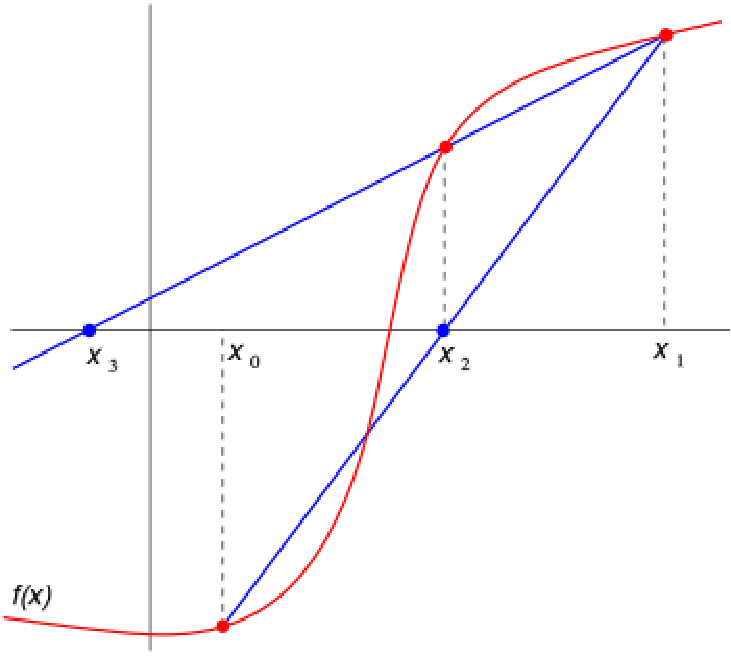
\includegraphics[scale=0.75]{images/secant_method}
    \end{center}
\end{frame}

%SLIDE 4
\begin{frame}{\hspace{50mm}Secant Method: Pseudocode}
    % go check out minted and listing packages
    \begin{algorithmic}[1]
        \Function{Secant}{$f, x_0, x_1, M, \delta, \epsilon$}
            \Let{$xvals_0$}{$x_0$}; $xvals_1 \gets x_1$
            \Let{$fvals_0$}{$f(xvals_0)$}; $fvals_1 \gets f(xvals_1)$
            \State \textbf{output} $0,$ $xvals_0$, $fvals_0$
            \State \textbf{output} $1,$ $xvals_1$, $fvals_1$
            \For{$k = 2 \textbf{ to } M$}
                \If{$\abs{fvals_{k-2}} > \abs{fvals_{k-1}}$}
                    \State $xvals_{k-2} \leftrightarrow xvals_{k-1}$; $fvals_{k-2} \leftrightarrow fvals_{k-1}$
                \EndIf
                \Let{$xvals_k$}{$xvals_{k-2}-fvals_{k-2}\cdot\dfrac{xvals_{k-1}-xvals_{k-2}}{fvals_{k-1}-fvals_{k-2}}$}
                \Let{$xvals_{k-1}$}{$xvals_{k-2}$}
                \Let{$fvals_{k-1}$}{$fvals_{k-2}$}
                \Let{$fvals_{k}$}{$f(xvals_{k})$}
            \EndFor
            \State \Return{$xvals, fvals$}
        \EndFunction
    \end{algorithmic}
\end{frame}

%ERROR ANALYSIS FRAME 1
\begin{frame}{\hspace{50mm}Secant Method: Error Analysis}
	\bi
		\item Our goal will be to estimate the $n+1^{th}$ error term based on the $n^{th}$ error term and the $n-1^{th}$ error term. First, note that the error $e_n=x_n-r$.
		\pause
		\item Using the definition of the secant method, we have
			\begin{align*}
				e_{n+1}&=x_{n+1}-r\\
				&=\frac{f(x_n)x_{n-1}-f(x_{n-1})x_n}{f(x_n)-f(x_{n-1})}-r.
			\end{align*}
		\pause
		\item We can substitute $x_n-r=e_n$ from the definition of our error and then simplify to give us
			\begin{align*}
				e_{n+1}&=\frac{f(x_n)e_{n-1}-f(x_{n-1})e_n}{f(x_n)-f(x_{n-1})}.
			\end{align*}
	\ei
\end{frame}

%ERROR ANALYSIS FRAME 2
\begin{frame}{\hspace{50mm}Secant Method: Error Analysis}
	\bi
		\item We can then remove a factor of $e_ne_{n-1}$ and insert a factor of $(x_n-x_{n-1})$ to give
			\begin{equation}\label{factor}
				e_{n+1}=\left[\frac{x_n-x_{n-1}}{f(x_n)-f(x_{n-1})}\right]\cdot\left[\frac{f(x_n)/e_n-f(x_{n-1})/e_{n-1}}{x_n-x_{n-1}}\right]\cdot e_ne_{n-1}.
			\end{equation}
		\pause
		\item Remember this equation (or write it down if you can't memorize this). It's important. 
		\pause
		\item We wish to bound $f(x_n)$ and $f(x_{n-1})$ in order to estimate our error in terms of a constant. So, first, note that Taylor's theorem gives us
			\begin{align*}
				f(x_n)&=f(r+e_n)\\
				&=f(r)+e_nf^\prime(r)+\dfrac{1}{2}e^2_nf^{\prime\prime}(r)+\mathcal{O}(e^3_n).
			\end{align*}
	\ei
\end{frame}

%ERROR ANALYSIS FRAME 3
\begin{frame}{\hspace{50mm}Secant Method: Error Analysis}
	\bi
		\item We are searching for a zero to the function, so clearly $f(r)=0$. Thus,
			\begin{align*}
				\dfrac{f(x_n)}{e_{n}}=f^\prime(r)+\frac{1}{2}e_nf^{\prime\prime}(r)+\mathcal{O}(e^2_n).
			\end{align*}
		\pause
		\item If we change the index from $n$ to $n-1$, we see that
			\begin{align*}
				\dfrac{f(x_{n-1})}{e_{n-1}}=f^\prime(r)+\frac{1}{2}e_{n-1}f^{\prime\prime}(r)+\mathcal{O}(e^2_{n-1}).
			\end{align*}
		\pause
		\item Subtracting the previous two equations yields 
			\begin{align*}
				\dfrac{f(x_n)}{e_n}-\dfrac{f(x_n)}{e_{n-1}}=\frac{1}{2}(e_n-e_{n-1})f^{\prime\prime}(r)+\mathcal{O}(e^2_{n-1}).
			\end{align*}
	\ei
\end{frame}

%ERROR ANALYSIS FRAME 4
\begin{frame}{\hspace{50mm}Secant Method: Error Analysis}
	\bi
		\item Since $x_n-x_{n-1}=e_n-e_{n-1}$, we can divide each side of the previous equation by $x_n-x_{n-1}$ and get
			\begin{align*}
				\frac{\dfrac{f(x_n)}{e_n}-\dfrac{f(x_n)}{e_{n-1}}}{x_n-x_{n-1}}\approx\dfrac{1}{2}f^{\prime\prime}(r). %I forgot how to extend the division sign to make this look clearer
			\end{align*}
			
			This is splendid, because $\frac{1}{2}f^{\prime\prime}(r)$ is a constant. This is also true with $\frac{1}{f^{\prime}}(r)$...
		\pause
		\item Note that the quantity contained within the first set of brackets in Equation \eqref{factor} can be rewritten as
			\begin{align*}
				\frac{x_n-x_{n-1}}{f(x_n)-f(x_{n-1})}\approx\frac{1}{f^\prime(r)}.
			\end{align*}
		\bi
			\item For those who were imprudent, remember that Equation \eqref{factor} was $e_{n+1}=\left[\frac{x_n-x_{n-1}}{f(x_n)-f(x_{n-1})}\right]\cdot\left[\frac{f(x_n)/e_n-f(x_{n-1})/e_{n-1}}{x_n-x_{n-1}}\right]\cdot e_ne_{n-1}$.
		\ei
	\ei
\end{frame}

%ERROR ANALYSIS FRAME 5
\begin{frame}{\hspace{50mm}Secant Method: Error Analysis}
	\bi 
		\item Thus, we have shown that %I think we should delineate this
			\begin{align*}
				e_{n+1}\approx\frac{1}{2}\cdot\frac{f^{\prime\prime}(r)}{f^\prime(r)}e_ne_{n-1}=Ce_ne_{n-1}.
			\end{align*}
		\pause
		\item Note that this is similar to the error in Newton's method, which was
			\begin{align*}
				e_{n+1}=\frac{1}{2}\cdot\frac{f^{\prime\prime}(\xi_n)}{f^\prime(x_n)}e^2_n\approx\frac{1}{2}\frac{f^{\prime\prime}(r)}{f^\prime(r)}e^2_n=Ce^2_n.
			\end{align*}
	\ei
\end{frame}

%APPLICATION OF THE SECANT METHOD IN FINANCE
\begin{frame}{\hspace{50mm}Secant Method: Implementation}
	\bi
		\item Code!
	\ei
\end{frame}

\end{document}

